\documentclass[../main.tex]{subfiles}
\graphicspath{{\subfix{../images/}}}


\begin{document}
% AIS
%%%%%%%%%%%%%%%%%%%%%%%%%%%%%%%%%%%%%%%%%%%%%%%%%%%%%%%%%%%%%%%%%%%%%%%%%%%%%%%
Vessels navigating the Baltic Sea

Importance of maritime traffic globally and timely operation


\subsection{Automatic identification system}

Automatic identification system (\textit{AIS}) was introduced by the International Maritime Organization (\textit{IMO}) in the early 2000's in accordance with the Safety of Life at Sea (\textit{SOLAS}) treaty as an open communication tool for all maritime traffic. The main objectives of the treaty is to improve the safety of life at sea, protection of the marine environment and safety and efficiency of navigation \cite{IMO_2015}. In its general operating form, AIS operates on two VHF channels and all vessels or base stations within the vessels transmission range receive the messages transmitted and vice versa the vessel receives all messages broadcasted in its receiving range. The broadcasting is based on Self-organized Time Division Multiple Access (\textit{(S)TDMA}) with a minimum of 2000 time slots per minute broadcasting capacity rate and the ship-to-ship communication for closer vessels takes precedence over vessels farther away which allows for sharing time slots, and thus overloading the available time slots \cite{IMO_2015}.

The IMO requires in accordance with regulation V/19 of SOLAS, that all vessels with a gross tonnage of 300 or more on international voyages, cargo vessels of 500 gross tonnage or more not on international voyages and all passenger vessel disregarding the gross tonnage to be equipped with an AIS. Further, the EU requires new-built fishing vessels longer than 15 meters to be fitted with an AIS from November 2010 and existing vessels to install an AIS May 2014 at the latest \cite{EU_2011}. There are two types of AIS Class A and Class B. Class A transceiver are the more common and are compliant with the IMO regulations whereas Class B transceivers are not subject to the full IMO AIS requirements. Class B transceivers are typically simpler, of lower cost and installed on smaller vessels of one's own choosing for improving the situational awareness. Class A transceivers take precedence over Class B transceivers when broadcasting.

The vessels onboard sensors and positioning systems interface with the AIS to allow for communicating the status of the vessel, both static and dynamic information. AIS also allows for voyage related information and safety-related information to be transmitted via the system, see Table \ref{tab:ais-data}. The AIS guidelines requires that there is a minimum display and keyboard for input and receive of data, for updating information manually and retrieving data received via AIS.

The information received by the AIS does not provide the full situational picture of the vessels surroundings and should only be used as a navigational and situational awareness aid.

\begin{figure}[H]
\centering
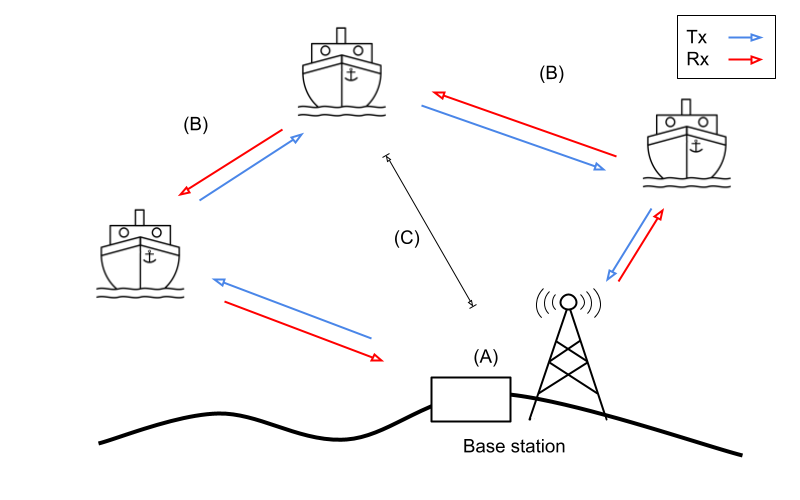
\includegraphics[scale=.5]{AIS-SOP.png}
\caption{(A) Base station transmits information about other vessels, port data and possible hazards. Base station receives information from all vessels in range. (B) Ship-to-ship communication. Vessel broadcasts its current state (identifier, speed over ground, course over ground etc.) and receives data from all vessels in range, only limited by the number of possible time slots available. (C) Vessel outside range of transmitting AIS data to the base station still transmits information to other vessels.}
\label{fig:ais-sop}
\end{figure}

The AIS integrated checks for data integrity, built-in integrity test (\textit{BIIT}), is not capable of validating data, for example a non-functional sensor will report as not available to the AIS.

The information available to transmit over AIS is divided into three groups static, dynamic and voyage-related.

\begin{table}[H]
\centering
\begin{tabular}{|m{5cm}|m{9cm}|}
\hline
\rowcolor[HTML]{C0C0C0} 
\multicolumn{1}{|c|}{\cellcolor[HTML]{C0C0C0}\textbf{Data}}  & \multicolumn{1}{c|}{\cellcolor[HTML]{C0C0C0}\textbf{Description}}                 \\ \hline
\rowcolor[HTML]{C0C0C0} 
\textbf{Static}                                              &                                                                                   \\ \hline
Maritime Mobile Service Identity (MMSI)                      & Set on installation, can change during vessels operational lifespan               \\ \hline
\rowcolor[HTML]{EFEFEF} 
Call sign and name                                           & Set on installation, can change during vessels operational lifespan               \\ \hline
IMO number                                                   & Set on installation                                                               \\ \hline
\rowcolor[HTML]{EFEFEF} 
Length and beam                                              & Set on installation or if changed                                                 \\ \hline
Type of ship                                                 & Selected from list of predefined values                                           \\ \hline
\rowcolor[HTML]{EFEFEF} 
Location of electronic positioning system                    & Set on installation, can be changed                                               \\ \hline
\rowcolor[HTML]{C0C0C0} 
\textbf{Dynamic}                                             &                                                                                   \\ \hline
Ships position with accuracy indication and integrity status & Automatically updated from the position sensor                                    \\ \hline
\rowcolor[HTML]{EFEFEF} 
Position time stamp in UTC                                   & Automatically updated from the main position sensor                               \\ \hline
Course over ground (COG)                                     & Automatically updated from the main position sensor if available                  \\ \hline
\rowcolor[HTML]{EFEFEF} 
Speed over ground (SOG)                                      & Automatically updated from the main position sensor                               \\ \hline
Heading                                                      & Automatically updated from the vessels heading sensor                             \\ \hline
\rowcolor[HTML]{EFEFEF} 
Navigational status                                          & Manually entered by the OOW as needed                                             \\ \hline
Rate of turn (ROT)                                           & Automatically updated from the vessels ROT sensor or from the vessels gyro        \\ \hline
\rowcolor[HTML]{C0C0C0} 
\textbf{Voyage-related}                                      &                                                                                   \\ \hline
Draught                                                      & Manually entered at the start of the voyage                                       \\ \hline
\rowcolor[HTML]{EFEFEF} 
Hazardous cargo (type)                                       & Manually entered at the start of the voyage confirming the presence of such cargo \\ \hline
Destination and ETA                                          & Manually entered at the start of the voyage and updates as needed                 \\ \hline
\rowcolor[HTML]{EFEFEF} 
Route plan (waypoints)                                       & Manually entered at the start of the voyage                                       \\ \hline
\rowcolor[HTML]{C0C0C0} 
\textbf{Safety-related}                                      &                                                                                   \\ \hline
Short safety-related messages                                & Free format manually entered broadcasted to specific receiver or all vessels      \\ \hline
\end{tabular}
\caption{AIS data content and description, from \cite{IMO_2015}.}
\label{tab:ais-data}
\end{table}

\subsubsection{Estimated Time of Arrival}

Estimated time of arrival is the estimated time when a vessel will reach its destination, typically transmitted to the correct authorities 24 to 72 hours before arrival \cite{Veenstra_2021, EU_2009}. The means of communicating this ETA varies and the accuracy of the ETA is not guaranteed to be within any margin of error. Ports, being very complex infrastructures with many moving parts, has to operate with certain uncertainties of vessels arrival times and required demands and it is essential to plan port operations for a 24-hour period at a minimum \cite{Fancello_2011}. All uncertainties that can delay or alter any operations at port are therefore a risk.

\subsection{HELCOM dataset}

The HELCOM dataset covers the period from January 2009 to December 2019. Each month for each year is stored as its own comma separated value \textit{.csv} file.

The AIS data in the HELCOM dataset is already processed to some extent compared too raw AIS data, see example of raw AIS data in Section \textbf{ref to raw ais}.

Describe the features and quirks with the HELCOM dataset as it is a processed dataset that contains AIS data already processed from the raw format. Merging of A and B AIS message types

HELCOM dataset has no ETA entries meaning to use this dataset for ETA prediction the ATA is calculated for all points on the route until the vessel has arrived, the true arrival time. Can't compare vessels ETA with the estimation but knows the estimated time left 

Showing examples of the data as plots of the Baltic, also shows the area covered

\begin{figure}[H]
\centering
\includegraphics[scale=.6]{heatmap-train-data-13-03.png}
\caption{Heatmap the Baltic Sea with a limit of more than 10 unique messages per grid cell.}
\label{fig:heatmap}
\end{figure}


\subsubsection{Description of HELCOM dataset features}

The HELCOM dataset have twelve unique features for each entry described in Table \ref{tabl:HELCOM-features}. The features are static, dynamic and voyage-related AIS data merged from multiple sources.

\begin{table}[H]
\centering
\begin{tabular}{|l|m{7cm}|l|}
\hline
\textbf{Name} & \textbf{Description}                                                  & \textbf{Value}             \\ \hline
timestamp     & Unix epoch time in milliseconds when AIS message was created          & Min 1230768000000          \\ \hline
mmsi          & Maritime Mobile Service Identities, unique for each vessel can change & 9 digits long              \\ \hline
lat           & Latitude position when AIS message was generated                      & Coordinate in WGS 84       \\ \hline
long          & Longitude position when AIS message was generated                     & Coordinate in WGS 84       \\ \hline
sog           & Speed over ground in knots                                            & 0.1 knot resolution        \\ \hline
cog           & Course over ground in degrees relative to true north                  & 0.1 degrees                \\ \hline
draught       & Vertical distance from waterline to the keel                          & 0.1 meters                 \\ \hline
dimBow        & Reference point for position of positioning system on the vessel      & Meters from bow            \\ \hline
dimPort       & Reference point for position of positioning system on the vessel      & Meters from port side      \\ \hline
dimStarboard  & Reference point for position of positioning system on the vessel      & Meters from starboard side \\ \hline
dimStern      & Reference point for position of positioning system on the vessel      & Meters from stern          \\ \hline
imo           & Unique identifier for each vessel, does not change                    & 7 digit identifier         \\ \hline
\end{tabular}
\caption{Variables in HELCOM data set and description.}
\label{tabl:HELCOM-features}
\end{table}

\subsubsection{Statistical information}

Unevenness of the recorded messages (time intervals distribution even) but large gaps in routes. Reasons can be merging of many databases, preprocessing of the data to unify the records. The number of "good" valid routes for training is much lower than the total number of routes. Some of that could be handled by generating routes (data) where there are gaps. In a realistic dataset with AIS data there are going to be faulty data and missing, so HELCOM data is quite accurate to real data without generating missing data.



Vessels physical features and the grouping of different vessels by size. In Figure \ref{fig:vessel-classes} an example of one year of unique vessels which have visited the port of Naantali can be seen. 

\begin{figure}[H]
\centering
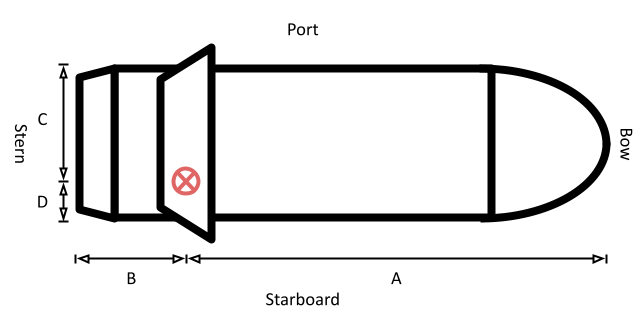
\includegraphics[scale=.5]{vessel-class-definition.png}
\caption{Vessel class definition from HELCOM data, the positioning system marked with red. A is \textit{dimStern}, B is \textit{dimBow}, C is \textit{dimPort} and D is \textit{dimStarboard}.}
\label{fig:vessel-class-def}
\end{figure}

\begin{figure}[H]
\centering
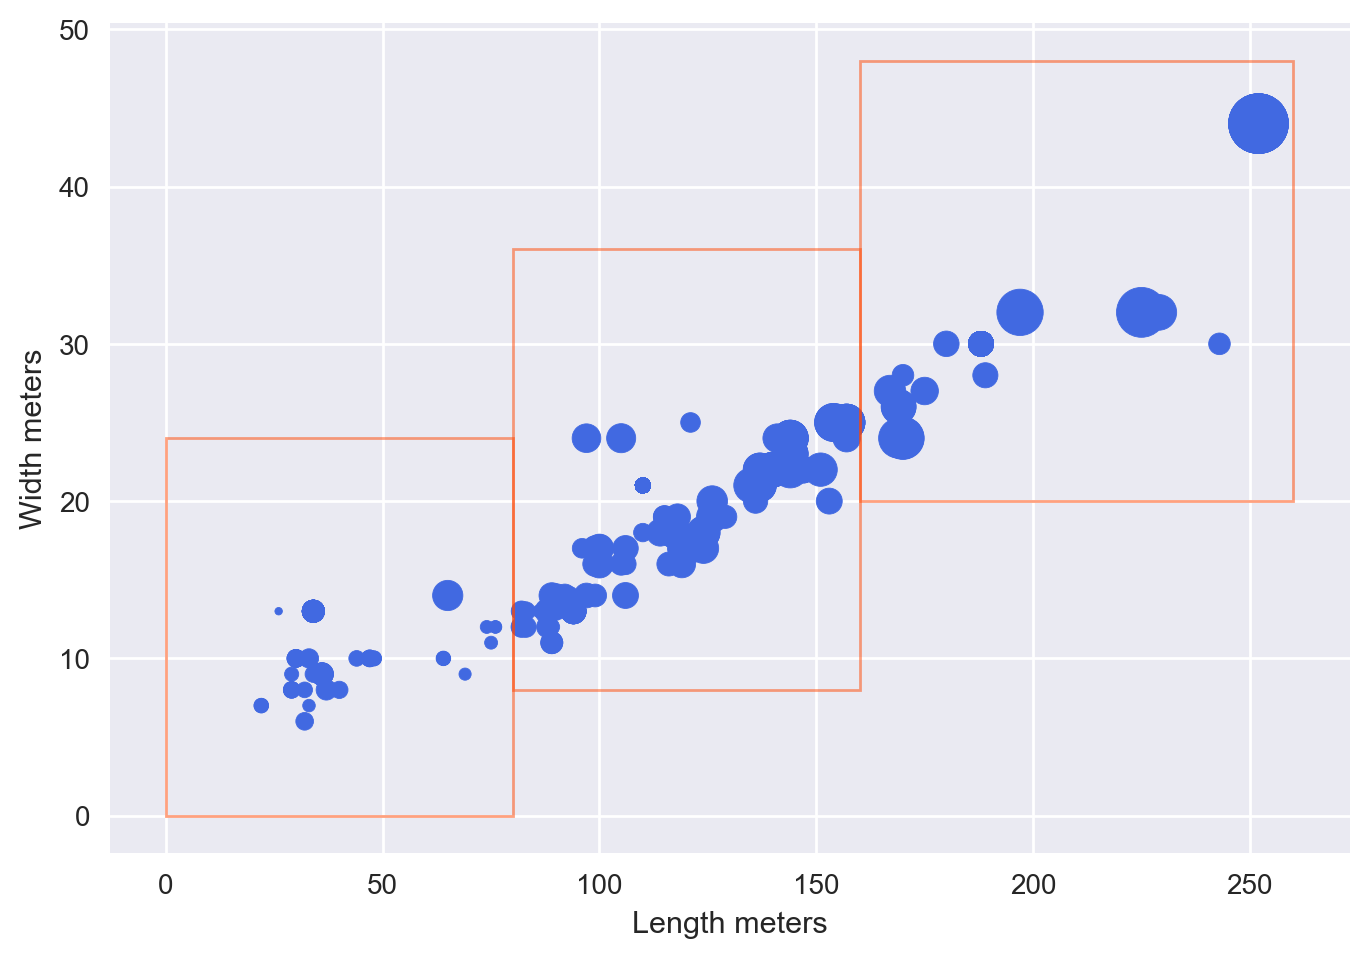
\includegraphics[scale=.5]{2015_ship_class.png}
\caption{Defined vessel classes and distribution of all unique vessels for the year 2015. Size of the circle is related to the draught of the vessel.}
\label{fig:vessel-classes}
\end{figure}


\subsection{Port of Naantali}

The Port of Naantali is a rather important and busy port in the Baltic Sea. With a reported total of over 8 million tonnes of cargo passing through the port and over 1,000 port calls during 2020 its logistical importance is of significance \cite{PoN_2021}. 

This is also recognised in the HELCOM data by the amount of the data that has any connections to the Port of Naantali.

\begin{table}[H]
\centering
\begin{tabular}{|l|c|c|c|c|c|c|c|c|c|c|}
\hline
\rowcolor[HTML]{C0C0C0} 
\multicolumn{1}{|r|}{\cellcolor[HTML]{C0C0C0}\textbf{Year}} & \textbf{2009} & \textbf{2010} & \textbf{2011} & \textbf{2012} & \textbf{2013} & \textbf{2014} & \textbf{2015} & \textbf{2016} & \textbf{2017} & \textbf{2018} \\ \hline
\textbf{\% of data}                           & 8.21          & 7.16          & 7.30          & 13.19         & 12.30         & 12.30         & 12.30         & 10.17         & 10.87         & 10.61         \\ \hline
\end{tabular}
\caption{Total amount of vessel data with connection to the Port of Naantali for each year of the HELCOM data.}
\label{tab:HELCOM-data-percent}
\end{table}

This data is the complete timeline for each vessel that has at any point during the years visited the Port of Naantali. Only a fraction of this data is actual viable data for the routes, described in \textbf{SECTION REFERENCE}.

The port is defined by manually defining a area that covers the whole operational area of the port, to include all berths and the possible routes to approach the port. Port of Naantali is for all vessels except small pleasure boats approachable from one direction, see Figure \ref{fig:FINLI-box}. This bounding box in red in Figure \ref{fig:FINLI-box} is what defines the area of when a vessel has entered the port. 
\begin{figure}[H]
\centering
\includegraphics[scale=.5]{FINLI_definition.png}
\caption{Defined bounding area for the Port of Naantali outlined in red. A small sample of the incoming routes shown in blue.}
\label{fig:FINLI-box}
\end{figure}



\end{document}